\documentclass[a4paper,11pt]{article}
% Various packages
\usepackage{siunitx}
\usepackage[utf8]{inputenc} % æøå
\usepackage[T1]{fontenc} % mere æøå
\usepackage[danish]{babel} % orddeling
\usepackage{verbatim} % så man kan skrive ren tekst
\usepackage{graphicx}
\graphicspath{{assets/}}
\usepackage{a4wide}
\usepackage{url}
\usepackage[left=2cm,top=2cm,bottom=1.5cm,right=2cm]{geometry}
\usepackage{amsmath}
\usepackage{amssymb}
\usepackage{amsthm}
\usepackage{wrapfig}
\usepackage{fixme}
\usepackage{color}
\usepackage{pstricks}
\usepackage{pdfpages} % include pdf
\usepackage{float} % Use [H] in figures
\usepackage{subcaption} % For subfigures
\usepackage{color} % May be necessary if you want to color links
\usepackage{hyperref} % Make references clickable
\usepackage[nameinlink,capitalize]{cleveref} % Make eq:refs be in style (1)
\usepackage[linesnumbered, commentsnumbered, lined, ruled, vlined,
%noend  % Have no ⌊-like symbol to indicate end of scope in pseudocode
]{algorithm2e} % Doc: https://goo.gl/6bC1qZ

% Ændr på navnene der vises når man bruger \autoref{label}
\def\sectionautorefname{Sektion}
\renewcommand{\equationautorefname}{Ligning}
\def\figureautorefname{Figur}
\AtBeginDocument{\renewcommand{\ref}[1]{\autoref{#1}}}

% Sæt \ref{} til at kalde \autoref{}
\AtBeginDocument{\renewcommand{\ref}[1]{\autoref{#1}}}

% Ændr ''*'' i math-felter til \cdot
\DeclareMathSymbol{*}{\mathbin}{symbols}{"01}

% Sæt farver for interne referencer og links
\definecolor{darkblue}{RGB}{25,25,112}
\hypersetup{
	colorlinks=true,    %set true if you want colored links
	linktoc=all,        %set to all if you want both sections and subsections linked
	linkcolor=darkblue, %choose some color if you want links to stand out
	filecolor=blue,     %
	citecolor=black,    %
	urlcolor=cyan,      %
}

% Set indentation to 0:
\setlength\parindent{0pt}

% Keywords relateret til algorithm2e pakken
\newcommand{\True}{\textbf{true}}\newcommand{\False}{\textbf{false}}
\SetStartEndCondition{ }{}{}%
\SetKwProg{Fn}{def}{\string:}{}
\SetKw{KwTo}{to}
\SetKwFor{For}{for}{}{}% 
\SetKwFor{ForEach}{foreach}{}{}% 
\SetKwIF{If}{ElseIf}{Else}{if}{}{elif}{else}{end}% 
\SetKwFor{While}{while}{}{end}\SetKwProg{Fn}{}{}{}
\SetKwInOut{Input}{input}\SetKwInOut{Output}{output}
\setlength{\algomargin}{3em}\DontPrintSemicolon

\newcommand{\longspace}{{\ \ \ \ \ \ \ \ \ \ \ \ \ \ }}
\renewcommand{\P}{{\mathbb P}}
\newcommand{\parfrac}[1]{\frac{\partial}{\partial #1}}
\renewcommand{\num}{{\textrm{num} }}
\newcommand{\size}{{\textrm{size} }}
\newcommand{\ift}{{\textrm{if } }}

% Dynamiske (), <>, ceil, floor
\newcommand{\p}[1]{\left( #1 \right)}
\newcommand{\pbig}[1]{\big( #1 \big)}
\newcommand{\pBig}[1]{\Big( #1 \Big)}
\newcommand{\pbigg}[1]{\bigg( #1 \bigg)}
\newcommand{\larr}[1]{\left< #1 \right>}
\newcommand{\ceil}[1]{\left\lceil #1 \right\rceil}
\newcommand{\floor}[1]{\left\lfloor #1 \right\rfloor}


% Squiggly arrows
\DeclareFontFamily{U} {MnSymbolC}{}

\DeclareFontShape{U}{MnSymbolC}{m}{n}{
	<-6> MnSymbolC5
	<6-7> MnSymbolC6
	<7-8> MnSymbolC7
	<8-9> MnSymbolC8
	<9-10> MnSymbolC9
	<10-12> MnSymbolC10
	<12-> MnSymbolC12}{}
\DeclareFontShape{U}{MnSymbolC}{b}{n}{
	<-6> MnSymbolC-Bold5
	<6-7> MnSymbolC-Bold6
	<7-8> MnSymbolC-Bold7
	<8-9> MnSymbolC-Bold8
	<9-10> MnSymbolC-Bold9
	<10-12> MnSymbolC-Bold10
	<12-> MnSymbolC-Bold12}{}

\DeclareSymbolFont{MnSyC} {U} {MnSymbolC}{m}{n}

\DeclareMathSymbol{\MNrhd}{\mathbin}{MnSyC}{76}
\DeclareMathSymbol{\MNlhd}{\mathbin}{MnSyC}{78}
% =============================================
\DeclareFontFamily{U} {MnSymbolD}{}

\DeclareFontShape{U}{MnSymbolD}{m}{n}{
	<-6> MnSymbolD5
	<6-7> MnSymbolD6
	<7-8> MnSymbolD7
	<8-9> MnSymbolD8
	<9-10> MnSymbolD9
	<10-12> MnSymbolD10
	<12-> MnSymbolD12}{}
\DeclareFontShape{U}{MnSymbolD}{b}{n}{
	<-6> MnSymbolD-Bold5
	<6-7> MnSymbolD-Bold6
	<7-8> MnSymbolD-Bold7
	<8-9> MnSymbolD-Bold8
	<9-10> MnSymbolD-Bold9
	<10-12> MnSymbolD-Bold10
	<12-> MnSymbolD-Bold12}{}

\DeclareSymbolFont{MnSyD} {U} {MnSymbolD}{m}{n}
\DeclareMathSymbol{\MNsim}{\mathbin}{MnSyD}{2}

% =============================================

\usepackage{amssymb,amsmath,stackengine}
\stackMath
\newcommand\rsquigarrow[1]{%
	\mathbin{\stackon[2pt]{\rightsquigarrow}{\scriptscriptstyle #1 }}
}

\author{Søren Mulvad, rbn601}

\title{Eksamensdisposition - Shortest Path}
\begin{document}
\maketitle

% Desuden skal hver studerende i gruppen udarbejde en individuel disposition for emnet "Binære søgetræer", som er et af emnerne til eksamen. En disposition skal bestå af de vigtigste punkter, du vil komme ind på til eksamen.
% Tænk på dispositionen som noget, du kan have med dig til eksamen, og som kan hjælpe dig med at huske, hvad du overordnet vil gennemgå til emnet "Binære søgetræer".
% Dispositionen skal ikke indeholde detaljerede beviser og lignende, men de mere overordnede delemner. Sørg for at gøre den kortfattet - f.eks. 5-10 punkter med stikord/-sætninger.


\begin{itemize}
\item \textbf{Motivation samt beskrivelse af problemet}

\item \textbf{Init og Relaxation}

\item \textbf{Bevis på at problemet udviser optimal delstruktur}

\item \textbf{Håndkørsel af \texttt{Bellman-Ford} algoritmen}

\item \textbf{Bevis af korrekthed af \texttt{Bellman-Ford} algoritmen}
\begin{itemize}
	\item Lemma 24.15 (Path-relaxation property)
	\item Lemma 24.2 (''Kortest-vej-estimatet'' er korrekt ved terminering)
	\item Theorem 24.4 (Korrekthed)
\end{itemize}

\item \textbf{Håndkørsel af \texttt{Dijkstra}'s algoritme}


\end{itemize}

%%%%%%%%%%%%%%%%%%%%%%%%%%%%%%%%%%%%%%%%%%%%%%%%%%%%%%%%%%%
%%%%%%%%%%%%%%%%%%%%%%%%%%%%%%%%%%%%%%%%%%%%%%%%%%%%%%%%%%%
%%%%%%%%%%%%%%%%%%%%%%%%%%%%%%%%%%%%%%%%%%%%%%%%%%%%%%%%%%%
\newpage
%%%%%%%%%%%%%%%%%%%%%%%%%%%%%%%%%%%%%%%%%%%%%%%%%%%%%%%%%%%
%%%%%%%%%%%%%%%%%%%%%%%%%%%%%%%%%%%%%%%%%%%%%%%%%%%%%%%%%%%
%%%%%%%%%%%%%%%%%%%%%%%%%%%%%%%%%%%%%%%%%%%%%%%%%%%%%%%%%%%
\section{Shortest Path}



\begin{itemize}
\item \textbf{Motivation samt beskrivelse af problemet}
\begin{itemize}
	\item Åbenlyst utrolig brugbart. Kan bruges både bogstaveligt til korteste vej, men man kan også have en vægtfunktion der er baseret på tid, materialeomkostninger, etc.\\
	Jeg vil her tale om ''Single Source Shortest Path'', altså når vi ønsker at finde den korteste vej fra en kildeknude til alle andre knuder i grafen.
	\item Givet en graf $G = (V, E)$ og en vægtfunktion $w(E)$, find da vejen $p$ fra f.eks. knude $u$ til $v$ med den laveste samlede vægt $w(p)$ således at $w(p) = \delta(u, v)$.
	\item Såfremt der ikke findes en vej fra $u$ til $v$ har vi defineret $\delta(u, v) = \infty$.
	\item Tegn denne graf:
	\begin{figure}[H]
		\begin{center}
			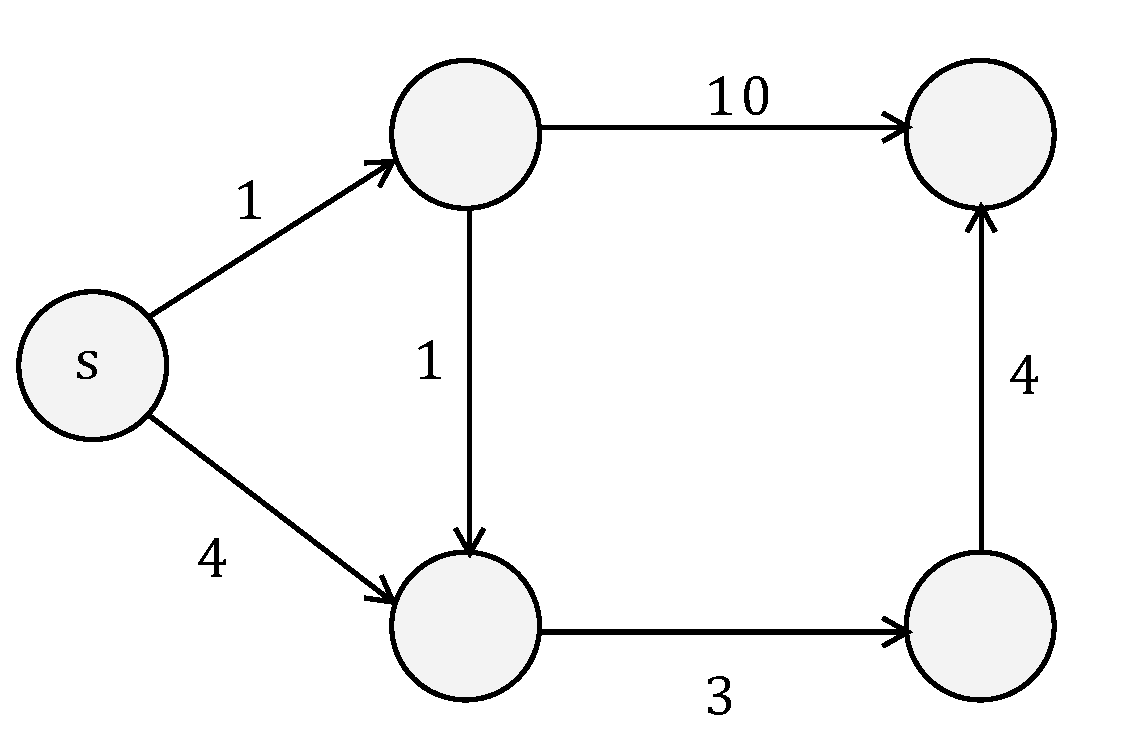
\includegraphics[width=0.4\textwidth]{graph.pdf}
		\end{center}
		%\caption{caption}
		\label{fig:graph}
	\end{figure}
\end{itemize}



\item \textbf{Init og Relaxation}
\begin{itemize}
	\item Vi indfører nu for alle knuder $v \in V$ en attribut $v.d$, som vi kan se som en upper bound for vægten af en kortest vej fra kildeknuden $s$ til $v$. Denne kaldes ''kortest-vej-estimat''.
	\item Derudover indfører vi attributten $v.\pi$ for alle knuder, som er dens forgænger (altså hvilken knude vi lige kom fra for at opnå den pt. korteste vej fundet).
	\item \texttt{Init} sætter for alle knuder $v.d = \infty$ og $v.\pi = NIL$.
	\item Vi indfører relaxtion for to knuder $u$ og $v$ der virker på den måde, at såfremt vi kan få et mindre ''kortest-vej-estimat'', så ændrer vi estimatet til dette og sætter $v$'s forgænger til $u$ på følgende måde:
	\begin{figure}[H]
		\begin{center}
			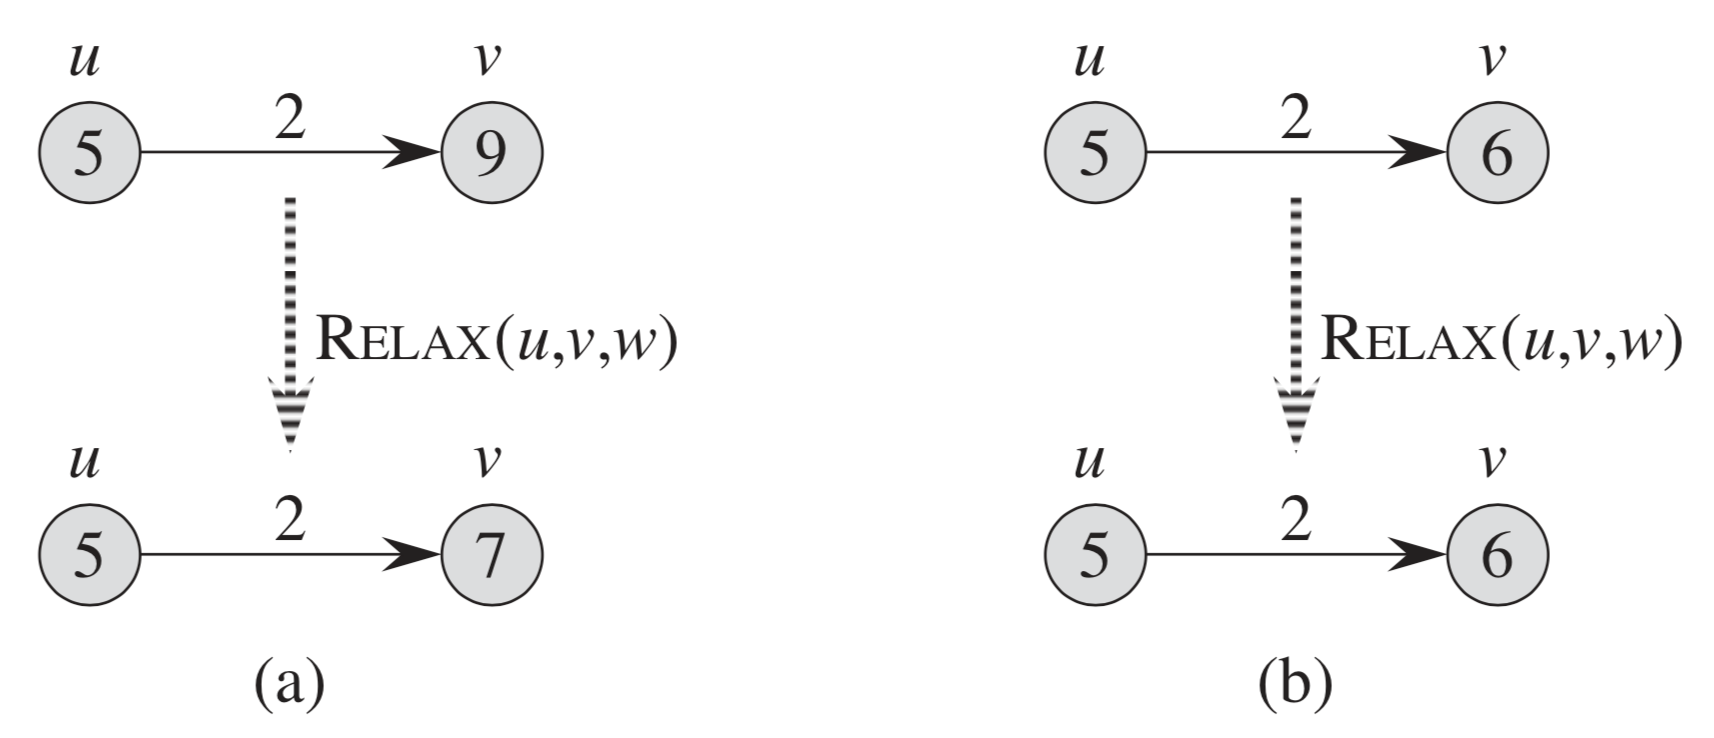
\includegraphics[width=0.65\textwidth]{relax.png}
		\end{center}
		\caption{Her relaxer vi kanten $(u, v)$. I (a) kan vi forbedre ''kortest-vej-estimateren'' og opdaterer derfor værdierne for $v$, mens vi ikke ændrer noget i (b).}
		\label{fig:relax}
	\end{figure}
\end{itemize}

\item \textbf{Bevis på at problemet udviser optimal delstruktur}
\begin{itemize}
	\item Lad $p = \left< v_0, v_{1}, ..., v_k \right>$ være en kortest vej fra $v_0$ til $v_k$.\\
	For ethvert $i$ og $j$ således at
	$$
	0 \leq i \leq j \leq k \quad\quad \textrm{lad} \quad\quad p_{ij} = \left< v_i, v_{i+1}, ..., v_j \right>
	$$
	være en delvej fra $v_i$ til $v_j$. Så er $p_{ij}$ en kortest vej fra $v_i$ til $v_j$.
	
	\item \textit{Bevis:} Lad os opløse vejen til
	$$
	v_0 \rsquigarrow{p_{0i}} v_i \rsquigarrow{p_{ij}} v_j \rsquigarrow{p_{jk}} v_k
	$$
	Så har vi, at
	$$
	w(p) = w(p_{0i}) + w(p_{ij}) + w(p_{jk})
	$$
	
	Lad os nu antage, at der findes en vej $p'_{ij}$ fra $v_i$ til $v_j$ med en vægt $w(p'_{ij}) < w(p_{ij})$. Men så ville vi få, at
	$$
	w(p) > w(p_{0i}) + w(p'_{ij}) + w(p_{jk})
	$$
	hvilket er en modstrid, da vi antog at $p$ var den korteste vej fra $v_0$ til $v_k$. 
\end{itemize}

%\item \textbf{Nogle ord om cykler og negative kanter}
%\begin{itemize}
%	\item Hvis der er en cykel med negativ vægt i vejen mellem to noder, så vil man kunne gå igennem denne uendeligt mange gange. Derfor vil den korteste vej i en sådan situation være $-\infty$.
%	\item I en kortest vej kan der ikke være positive vægt-cykler, da vi således kunne fjerne cyklen og få en kortere vej. Hvis vi har en cykel med 0-vægt vil vi også altid kunne fjerne den.
%	\item Der er som udgangspunkt ikke noget galt med negative kanter, det er problemet stadig veldefineret for. I Dijkstra's algoritme antager vi dog at ingen kanter er negative.	
%\end{itemize}

%\newpage
\item \textbf{Håndkørsel af \texttt{Bellman-Ford}}
\begin{itemize}
	\item Algoritme: \textit{(Ikke skriv op, men for forståelse)}\\
	\begin{algorithm}[H] \caption{MST-Kruskal} \label{alg:bellman}
		\SetKwFunction{func}{Bellman-Ford}%
		\SetKwFunction{Relax}{Relax}%
		\SetKwFunction{Init}{Initialize-Single-Source}%
		\Fn(){\func{G, w, s}}{
			\Init{G, s}\;
			\For{$i = 1 \ \KwTo \ |G.V| - 1$}{
				\ForEach{edge $(u, v) \in G.E$}{
					\Relax{u, v, w}\;
				}
			}
			\ForEach{edge $(u, v) \in G.E$}{
				\If{$v.d > u.d + w(u, v)$}{
					\Return FALSE\;
				}
			}
			\Return TRUE\;
		}
	\end{algorithm}\vspace{1em}

	Altså:\\
	Initialiser alle vægte\\
	Relax alle kanter $|V| - 1$ gange\\
	Test for alle kanter $(u, v)$ om $v.d > u.d + w(u,v)$ - hvis ja, returner \texttt{False}\\
	Ellers returner \texttt{True}.
	\begin{figure}[H]
		\begin{center}
			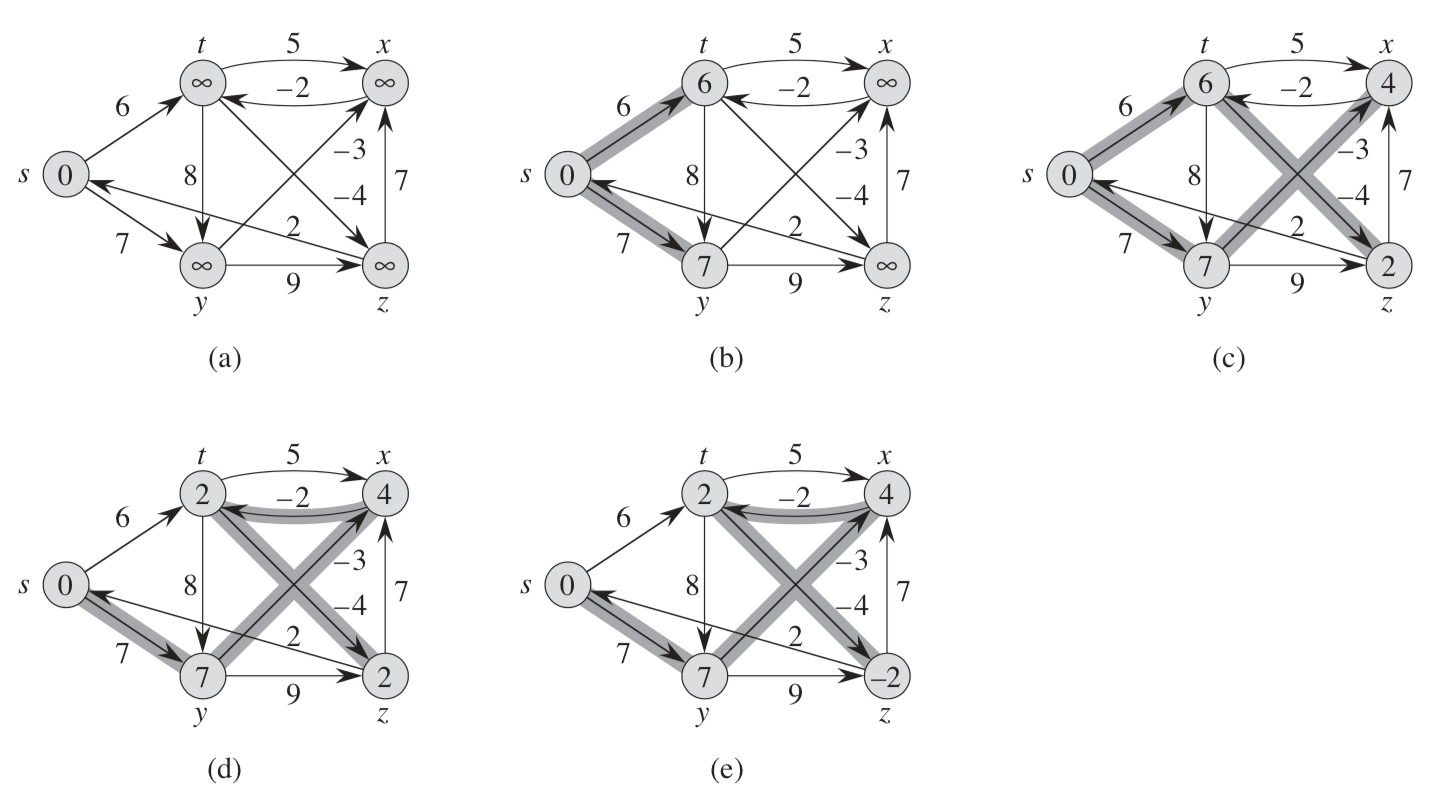
\includegraphics[width=0.75\textwidth]{bellman.png}
		\end{center}
		\caption{Illustration. Vær her opmærksom på, at kanterne relaxes i en bestemt rækkefølge og mellemresultaterne kunne se anderledes ud hvis de blev relaxet i en anden rækkefølge.}
		\label{fig:bellman}
	\end{figure}
	\item Køretiden for Bellman-Ford er $O(VE)$, da det største bidrag kommer fra vi går igennem alle $E$ kanter $V-1$ gange.
\end{itemize}

\item \textbf{Bevis af korrekthed af \texttt{Bellman-Ford}}
\begin{itemize}
	\item Tre dele: Path-relaxation property, Lemma 24.2, Theorem 24.4
	\item Path-relaxation property
	\begin{itemize}
		\item \textit{Def:} Givet vi har en kortest vej $p = \left< v_0, v_1, ..., v_k \right>$ fra $s = v_0$ til $v_k$. Så vil den sekvens af relaxation steps, som inkluderer i rækkefølge at relaxe
		$$
		(v_0, v_1), (v_1, v_2), ..., (v_{k-1}, v_k)
		$$
		medføre at $v_k.d = \delta(s, v_k)$. Dette gælder uanset om vi relaxer andre knuder indimellem.
		\item \textit{Bevis:} Induktionsbevis, hvor vi viser, at efter den $i$'te kant er relaxet har vi, at $v_i.d = \delta(s, v_i)$.
		\item For vores basis $i = 0$ ser vi det er sandt, da $v_0.d = s.d = 0 = \delta(s, s)$.
		\item For det induktive step antager vi, at $v_{i-1}.d = \delta(s, v_{i-1})$ og ser på hver der sker når vi relaxer kanten $(v_{i-1}, v_i)$. Her har vi en konvergensegenskab jeg ikke vil bevise som da siger, at $v_i.d = \delta(s, v_i)$. Denne lighed er vedligeholdt for hele tiden fremover. Hermed er det bevist.
	\end{itemize}
	\item Lemma 24.2 (''Kortest-vej-estimatet'' er korrekt ved terminering)
	\begin{itemize}
		\item \textit{Def:} Efter de $|V| - 1$ iterationer af for-loopet har vi, at $v.d = \delta(s, v)$ for alle knuder der kan nås fra kildeknuden (Vi antager at der ikke er nogle negative cykler).
		\item \textit{Bevis:} Tag udgangspunkt i enhver knude $v$ som kan nås fra $s$, og lad $p = \left< v_0, v_1, ..., v_k \right>$ hvor $v_0 = s$ og $v_k = v$ være en kortest vej fra $s$ til $v$. Fordi korteste veje er simple, så har vi at $p$ højest har $|V| - 1$ kanter, så:
		$$
		k \leq |V| - 1
		$$
		Vi relaxer netop alle kanter så mange gange, heriblandt kanten $(v_{i-1}, v_i)$ i den $i$'te iteration. Ved at tage udgangspunkt i path-relaxation property har vi da ved terminering, at:
		$$
		v.d = \delta(s, v)
		$$
	\end{itemize}
	\item Theorem 24.4 (Korrekthed af \texttt{Bellman-Ford})
	\begin{itemize}
		\item \textit{Def:} Hvis en graf $G$ ikke har nogle negative cykler, så returnerer algoritmen \texttt{True} og har beregnet en korteste vej korrekt til alle knuder fra kildeknuden.\\
		Hvis $G$ indeholder negative cykler, så returnerer algoritmen \texttt{False}.
		\item \textit{Bevis:} Først beviser vi det tilfælde, når $G$ ikke har negative cykler. Da har vi lige bevist Lemma 24.2, og har altså derfor for alle knuder at $v.d = \delta(s, v)$. Vi har en ''predecessor-subgraph property'' som jeg ikke vil bevise, men af den følger, at så vil deres forgænger-attributer være sat korrekt og vi herved får den korteste vej. Hvis knuden ikke kan nås fra kildeknuden, så har vi en anden egenskab, ''no path property'', som viser at $v.d = \infty$ hvilket er korrekt jf. vores definition.
		\item Herefter skal vi vise at den returnerer \texttt{True}.\\
		Når den terminerer har vi for alle knuder, at:
		\begin{align*}
		v.d &= \delta(s, v)\\
		    &\leq \delta(s, u) + w(u, v) \quad\quad \textrm{(pga. trekantsuligheden)}\\
		    &= u.d + w(u, v)
		\end{align*}
		Ingen af testene vil således returnere \texttt{False}, og derfor vil den returnere \texttt{True}.
		\item Nu beviser vi, at den returnerer \texttt{False} når der er en negativ cyklus i $G$. Lad os kalde denne cyklus $c = \left< v_0, v_1, ..., v_k \right>$, hvor $v_0 = v_k$. Så har vi at den totale vægt af $c$ er mindre end 0 pr. definition.\\
		Antag nu for modstrid, at Bellman-Ford returnerer \texttt{True}. Altså vil
		$$
		v_i.d \leq v_{i-1}.d + w(v_{i-1}, v_i) \quad\quad \textrm{(for $i = 1,2,...,k$)}
		$$
		Ved at summere ulighederne for cyklerne får vi:
		\begin{align}
		\sum_{i=1}^k v_i.d &\leq \sum_{i=1}^k \p{ v_{i-1}.d + w(v_{i-1}, v_i)  } \label{eq:first} \\
		                   &= \sum_{i=1}^k v_{i-1}.d + \sum_{i=1}^k w(v_{i-1}, v_i) \label{eq:second}
		\end{align}
		Men da vi har at $v_0 = v_k$ vil hver knude i $c$ indgå præcis én gang i både hvad der er på venstresiden i \cref{eq:first} og venstre led i \cref{eq:second}, og disse to udtryk er derfor lig hinanden. Derved får vi, at
		$$
		0 \leq \sum_{i=1}^k w(v_{i-1, v_i})
		$$
		Men vi antog netop, at vores cyklus var negativ, hvilket er en modstrid. Hermed er det bevist at algoritmen korrekt vil returnere \texttt{False} såfremt der er en negativ cyklus.
	\end{itemize}
\end{itemize}

\item \textbf{Håndkørsel af \texttt{Dijkstra}'s algoritme}
\begin{itemize}
	\item Antager alle kanter har en ikke-negativ vægt.
	\item Algoritme: \textit{(Ikke skriv op, men for forståelse)}\\
	\begin{algorithm}[H] \caption{Dijkstra} \label{alg:dijkstra}
		\SetKwFunction{func}{Dijkstra}%
		\SetKwFunction{Extract}{Extract-Min}%
		\SetKwFunction{Relax}{Relax}%
		\SetKwFunction{Init}{Initialize-Single-Source}%
		\Fn(){\func{G, w, s}}{
			\Init{G, s}\;
			$S = \emptyset$\;
			$Q = G.V$\;
			\While{$Q \neq \emptyset$}{
				$u = \Extract{Q}$\;
				$S = S \cup \{u\}$\;
				\ForEach{vertex $v \in G.Adj[u]$}{
					\Relax{u, v, w}\;
				}
			}
		}
	\end{algorithm}\vspace{1em}
	
	Altså:\\
	Initialiser alle vægte\\
	Løbende find knuden med lavest ''kortest-vej-estimat'' og relax alle dens kanter til omkringliggende knuder.
	\item Illustration:
	\begin{figure}[H]
		\begin{center}
			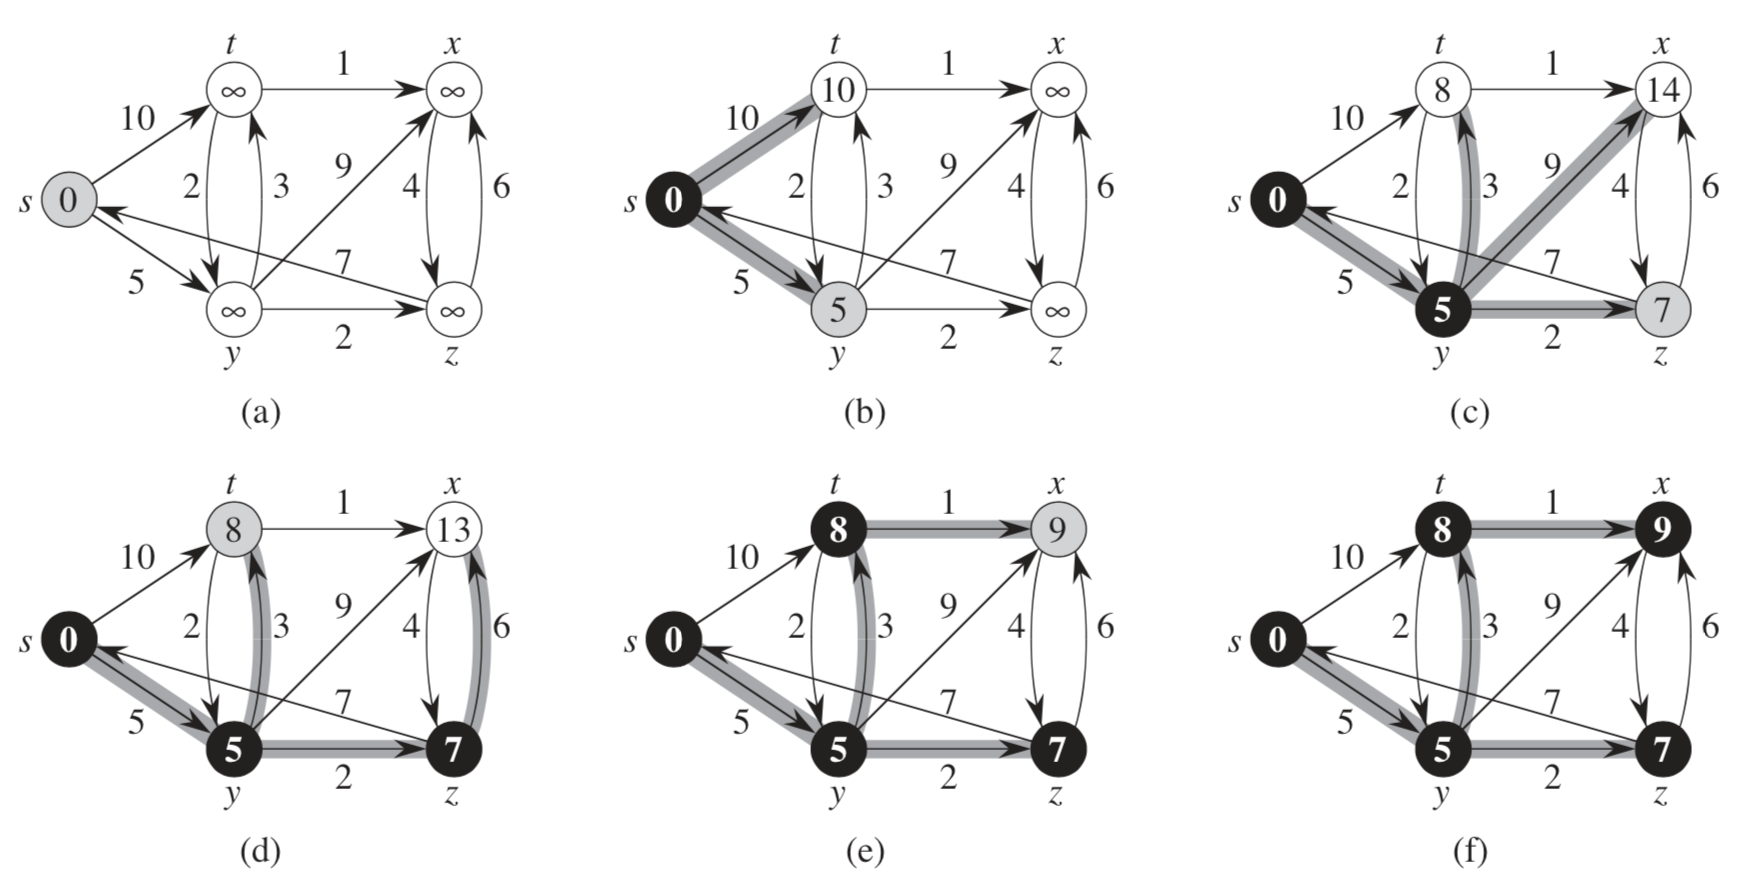
\includegraphics[width=0.8\textwidth]{dijkstra.png}
		\end{center}
		\caption{Dijkstras algoritme}
		\label{fig:dijkstra}
	\end{figure}
	
	
	\item Køretiden afhænger af hvilken underliggende datastruktur vi bruger, hvor Fibonacci Heaps er mest optimalt. Vi udfører
	\begin{enumerate}
		\item $|V|$ \texttt{Extract-Min} operationer som hver tager $O(\lg V)$ tid.
		\item $|E|$ \texttt{Decrease-Key} operationer (da vi kigger på alle kanter præcis én gang) som hver amortiseret tager $O(1)$ tid.
	\end{enumerate}
	
	Herved fås vi altså en samlet køretid:
	$$
	O(V \lg V + E)
	$$
\end{itemize}

\newpage
\item \textbf{Korrekthed af \texttt{Dijkstra}'s algoritme}
\begin{itemize}
	\item Det vi skal vise for at Dijkstra er korrekt, så skal vi vise, at når man tilføjer en knude til løsningsmængden $S$, så er det fordi vi allerede har fundet den korteste vej. Vi skriver løkkeinvarianten:\\
	
	\textit{Claim}: Når $u$ tilføjes til $S$ har vi at $u.d = \delta(s, u)$.\\
	
	\textit{Base case:}
	$$
	s.d = \delta(s, s) = 0
	$$\\
	
	\textit{Induktionsstep:}\\
	Vi bruger stærkt induktion, hvor vi antager at alle de knuder vi allerede har tilføjet til $S$ er den korteste vej.\\
	Antag nu for modstrid at vi tilføjer knuden $u$, men $u.d \neq \delta(s, u)$ - hvorved vi får følgende pr. upper bound property:
	$$
	u.d > \delta(s, u)
	$$
	Der må findes en vej fra $s$ til $u$, da hvis der ikke gjorde, så var den korteste vej uendelig pr. upper bound property (da hvis der ikke gjorde, så kunne den aldrig nogensinde blive uendelig pga. no path property).\\
	Når vi tilføjede den, så ville den altså allerede være lig den korteste vej. Så lad os sige at den korteste vej går gennem kanten $(x, y)$. Vi definerer $y$ til at være den første knude i stien fra $s$ til $u$ som ikke allerede er tilføjet til løsningsmængden $S$:\\\\
	\begin{figure}[H]
		\begin{center}
			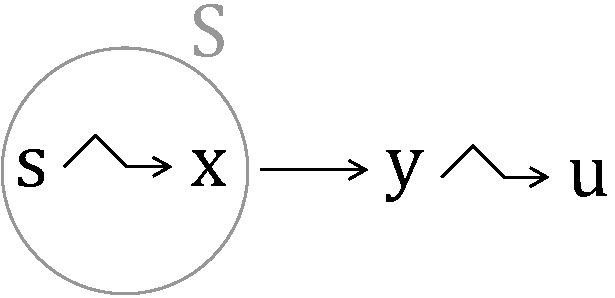
\includegraphics[width=0.4\textwidth]{dijkstra-proof.pdf}
		\end{center}
		%\caption{caption}
		\label{fig:proof}
	\end{figure}
	Dvs. at $x$ (som evt. godt kan være $s$) er i vores løsningssæt $S$, som pr. den stærke induktionsantagelse må have, at $x.d = \delta(s, x)$. Vi ved derudover, at da vi tilføjede $x$, så har vi relaxet alle udadgående kanter.\\
	Pr. convergence property betyder det, at $y.d = \delta(s, y)$.
	Derudover ved vi, at $y$ kommer før $u$ i den korteste vej til $u$. Da vi ikke har nogle negative kanter, så må den korteste vej til $y$ må være mindre end eller lig den korteste vej fra $s$ til $u$, hvilket er mindre end den distance vi har fundet til $u$ pr. vores modstridsantagelse:
	$$
	y.d = \delta(s, y) \leq \delta(s, u) < u.d
	$$
	Vi har nu både $y$ og $u$, og hvis de var ens, så havde vi allerede fundet den korteste vej til $u$ når vi tilføjer den. Derfor må de være forskellige. Men vi har tænkt os at tilføje $u$ til $S$, dvs.
	$$
	u.d \leq y.d
	$$
	(ellers ville vi være igang med at tilføje $y$ pr. Dijkstras algoritme).\\
	Vi ser nu, at vi får følgende ulighed hvilket er en modstrid, og derfor er Dijkstra korrekt:
	$$
	y.d < u.d \leq y.d
	$$
\end{itemize}


\item \textbf{Egenskaber}
\begin{itemize}
	\item \textbf{Trekantsulighed:} For enhver kant $(u, v) \in E$ har vi at $\delta(s, v) \leq \delta(s, u) + w(u, v)$.
	\item \textbf{Upper-bound property:} Vi har altid at $v.d \geq \delta(s, v)$ for alle knuder $v \in V$, og når $v.d$ får værdien $\delta(s, v)$ ændres den aldrig.
	\item \textbf{No-path property:} Hvis der ikke er nogen vej fra $s$ til $v$, så har vi altid at $v.d = \delta(s, v) = \infty$.
	\item \textbf{Konvergensegenskab:} Hvis $s \rsquigarrow{ } u \rightarrow v$ er en kortest vej for $u, v \in V$ og $u.d = \delta(s, u)$ på ethvert tidspunkt før vi relaxer kanten $(u, v)$, så vil $v.d = \delta(s, v)$ efter vi relaxer og for altid fremover.
	\item \textbf{Path-relaxation property:} Hvis $p = \left< v_0, v_1, ..., v_k   \right>$ er en kortest vej fra $s=v_0$ til $v_k$, og vi relaxer kanterne af $p$ i rækkefølgen $(v_0, v_1), (v_1, v_2), ..., (v_{k-1}, v_k)$, så vil $v_k.d = \delta(s, v_k)$. Dette holder uanset hvad vi relaxer i mellemtiden.
	\item \textbf{Predecessor subgrapgh-property:} Når $v.d = \delta(s, v)$ for alle $v \in V$, så er forgænger-delgrafen et kortest vej træ med rod i $s$.
\end{itemize}

\end{itemize}
\end{document}